\chapter{EMC Effect}	
\section{European Muon Collaboration}\label{sec:EMC}
\paragraph{}The European Muon Collaboration (EMC) performed a deep inelastic measurement with 120-280 GeV muons on iron and deuteron targets \cite{challenge}. The EMC studied the per nucleon normalized Fe/D structure function ratio versus the Bjorken scaling variable, $x$. The EMC expectations for this ratio originally was unity for $x$ between 0.05 and 0.7 \cite{CC}. The reasoning for this expectation was the belief that at large magnitude of $Q^2$ the interaction between protons and neutrons would not contribute to the total structure function of the nucleus. This was the understanding because the binding energy of a few MeV would not interferer with GeV scale of the DIS interaction \cite{Ajth}. The expected structure function for a nucleus could be written as:
\begin{equation}
F_2^A = N F_2^N + ZF_2^P.
\end{equation}
In this quasi-free nucleon picture, the nucleons are used to build up the nuclear structure ($F_2^A$) by summing up the neutron structure function ($F_2^N$) with the proton structure function($F_2^P$) for each nucleon. 



The EMC compared the extracted structure functions from iron and deuterium. Their results are shown in Figure \ref{EMCOld}. The $\frac{A}{D}$ structure function ratio showed an unexpected downward slope. This phenomenon was titled the EMC effect. This finding demonstrated to the EMC that their understanding of the nucleus was incorrect. A nucleon's structure function and thereby, the constituent quark distributions may be altered by the nucleus. 
\begin{figure}[h]
	\centering
	\caption{ Graph of the ratio of A/D structure functions vs $x$ from the EMC. \cite{CC,EM}.}
	\label{EMCOld}
	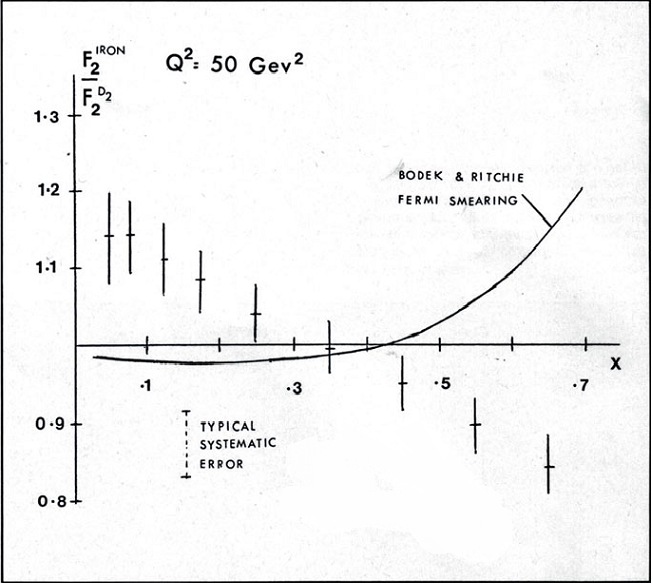
\includegraphics[width=10cm]{EMC.png} 
\end{figure} 

\paragraph{}Ever since the European Muon Collaboration discovered the depletion of quarks at high $x$ for A $>$2 nuclei, physicists have tried to discover its cause. Scientists at SLAC extracted structure function ratios for many nuclei including; $^4$He, $^9$Be, $^{12}$C, $^{27}$Al, $^{40}$Ca, $^{56}$Fe, $^{108}$Ag, and $^{197}$Au. There were slightly different results for each nucleus. The magnitude of the EMC effect, taken to be the A/D ratio at $x=0.6$, was found to be different for the various nuclei, and roughly scaled with the size or density of the nuclei. The NMC (New Muon collaboration), another group at CERN, gathered precise data in order to construct the inclusive cross section of deuterium and protons. BCDMS collaboration extracted data for N and Fe structure function ratios. Figure \ref{EMC3} shows some of the data from SLAC and BCDMS on the EMC effect for Iron and Cu. Figure \ref{EMC 1} shows this result from a recent JLab EMC measurement, most precise to date. Many models over the years have been able to reproduce the shape of the A/D ratios. These models can contain traditional nuclear physics effects like momentum distribution or pion-charge contributions. Some models also describe the EMC effect through quark momentum distribution or modification of the internal structure \cite{Norton, piler, arri, DF, gomez}. However, no single model has provided a complete picture of the possible underlying physics. Precise data from Jlab's E03-103 experiment has revitalized this research. This experiment focused on precision measurements in light nuclei and added $^{3}$He as a target nucleus. Instead of taking the A/D ratio at a certain $x$-value to be the magnitude of the EMC effect, this analysis looked at the slope instead. This eliminated sensitivity to normalization uncertainties.

\begin{figure}[h]
\centering
\caption{EMC effect from EMC, SLAC, and BCDMS \cite{Norton}}
\label{EMC3}
\centering
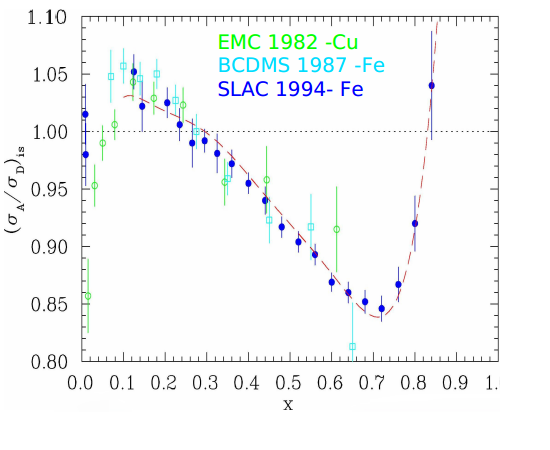
\includegraphics[width=10cm]{EMC3.png}
\end{figure}

\begin{figure}[h]
\centering
 \caption{ Graph of the ratio of A/D structure functions vs $x$ for Carbon \cite{CC}.}
 \label{EMC 1}
 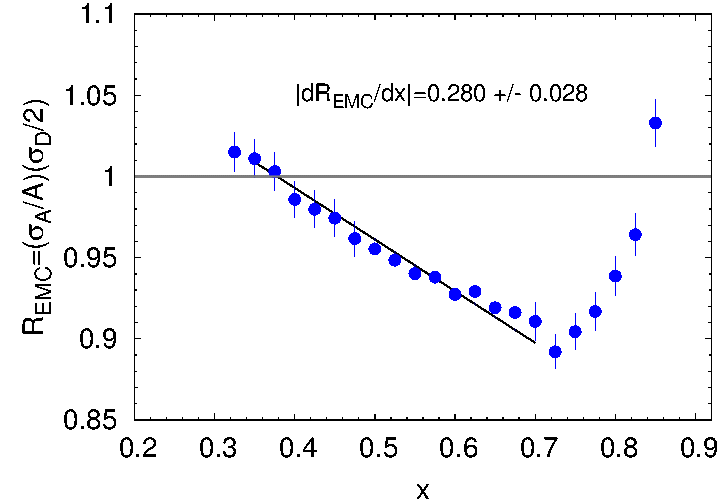
\includegraphics[width=10cm]{EMC1.png} 
 \end{figure} 
 

\paragraph{} In Figure , $^9$Be was found not to follow the previously observed scaling with nuclear density. This result from Jefferson Lab determined that the previous idea of a dependence on A or nuclear density in the EMC effect to be incorrect \cite{seeley}. This result spawned a drive to determine another explanation for the EMC effect and understand what clue the $^9$Be outlier was providing. The structure of this nucleus is made up of two high-density alpha particles and a single neutron \cite{ajppt}. The regions of higher density that are contained in a comparatively large volume may be able to explain why $^9$Be does not follow the expected trend. This suggests that the EMC effect could be a function of local nuclear density \cite{seeley}. 




\section{MARATHON}
Experiment E12-010-102, MARATHON (MeAsurement of the $F2^n$/$F_2^p$,$d$/$u$ RAtios and A=3 EMC Effect in Deep Inelastic Electron Scattering Off the Tritium and Helium MirrOr Nuclei), will use deep inelastic scattering off of the mirror nuclei $^3$H and $^3$He to measure the EMC effect for both $^3$H and $^3$He, to determine the ratio of the neutron to proton inelastic structure functions, and to find the ratio of the down to up quark distributions in the nucleon.

